\documentclass[12pt,a4]{article}

\usepackage{polski}
\usepackage[utf8]{inputenc}
\usepackage{graphicx}

\title{Raport do programu AJRES, krótkoterminowe przewidywanie długości doby}
\author{Łukasz Ślusarczyk}

\begin{document}

\maketitle
\tableofcontents
\clearpage

\section{Pobranie źródeł i instalacja}
Aby pobrać najnowszą wersję programu wpisz:\\
\begin{verbatim}git clone git@github.com:lucasso/ajres.git\end{verbatim}
Komenda ta utworzy w bieżącym katalogu podkatalog ``ajres'', a w nim można będzie znaleźć źródła programu.
Aby je skompilować należy wejści do katalogu ``ajres'' i wpisać:\\
\begin{verbatim}make\end{verbatim}
W przypadku błędów kompilacji sprawdź czy masz wszystkie wymagane przez program biblioteki.
Opis wymaganych bibliotek jest w rozdziale \ref{sec:wymagania_programu}
\section{Opis interfejsu użytkownika}
\subsection{Szybki start}
Aby uzyskac opis dostępnych opcji należy wpisać:\\
\begin{verbatim}./bin/ajres --help\end{verbatim}
Najprostszy sposób na wypróbowanie najprostszej sieci neuronowej do przewidywania długości dnia uzyskamy przez:\\
\begin{verbatim}./bin/ajres --plotPredictionError --plotInputData\end{verbatim}
Zebrane długości dnia zostana przepuszczone przez sieć złożoną z dwóch neuronów wejsciowych (w tym jeden jest neuronem
polaryzacji), dwóch neuronów ukrytych (w tym jeden jako polaryzacja) oraz jednego neuronu sprzeżenia zwrotnego z
opóźnieniem, który jest charakterystyczny dla sieci RMLP. Efekty działania programu znajdą się po jego zakończeniu w
katalogu ``out''. Plik \begin{verbatim}out/lod.png\end{verbatim} będzie zawierał dane wejściowe, zaś plik 
\begin{verbatim}out/predictionErrors.png\end{verbatim} błędy 
oszacowań kolejnych wartości przewidywanych przez sieć RMLP. Prócz tego znajdą się tam też pliki tekstowe z logami.
\subsection{Opis parametrów wejściowych}

\subsubsection{help} Wypisuje spis dostępnych opcji i kończy działanie programu.
\subsubsection{inputDelayNronsNum arg} Ustawia liczbę neuronów tej części warstwy wejściowej, która zawiara polaryzację,
wejście systemu i opóźnienia wejścia systemu. Nie może być mniejsza niż 2. Domyślna wartość to 2. Nie ma żadnego wpływu 
na działanie programu jeśli ajres jest w trybie ``ARCHITECTURE\_SEARCH'' 
(patrz rozdział \ref{sec:tryby_dzialania_programu}).
\subsubsection{outputDelayNronsNum arg} Ustawia liczbę neuronów tej części warstwy wejściowej, która odpowiada za
wprowadzenie do sieci opóźnionych sygnałów z wyjścia sieci. Może być dowolna, nawet 0, domyślnie jest 1.
\subsubsection{hiddenNronsNum arg} Ustawia liczbę neuronów warstwy ukrytej wliczając w to polaryzację. Liczba ta nie może
być mniejsza niż 2. Domyślna wartość to 2.
\subsubsection{searchForBestArchitecture arg} Domyślnie ajres działa w trybie ``SINGLE\_NET'' mode. Ta opcja przełącza tryb
na ``ARCHITECTURE\_SEARCH'' i jednocześnie określa zakres poszukiwań optymalnej architejtury sieci poprzed podanie
maksymalnej liczby neuronów w całej sieci. Minimalna akceptowalna wartość to 4. Nie ma wartości domyślnej.
Podanie tej opcji sprawia, że opcje inputDelayNronsNum, outputDelayNronsNum i hiddenNronsNum nie mają żadnego efektu.
\subsubsection{inputData arg} Lokalizacja pliku z historycznymi danymi orientacji przestrzennej ziemi w formacie IAU2000A.
Ten plik ściąga się razem z programem i nie ma potrzeby zmieniać tej opcji, ale oczywiście można. Domyślna wartość to:\\
\begin{verbatim}data/long/eopc04_IAU2000.62-now\end{verbatim}opis formatu jest na:\\
\begin{verbatim}http://www.iers.org/IERS/EN/DataProducts/
EarthOrientationData/eop.html?__nnn=true\end{verbatim}
\subsubsection{plotInputData} Flaga mówiąca czy wygenerować plik ``out/lod.png'' ilustrujący dane wejściowe.
\subsubsection{plotPredictionError} Flaga mówiąca czy wygenerować plik ``out/predictionErrors.png'' 
ilustrujący błędy prognozy.
\subsubsection{plotLearningFactorComputation} Generuje wykres funkcji celu w zależności od współczynnika uczenia przy 
każdym kroku, w którym zmieniane są wagi sieci. Bardzo spowalnia działanie programu. Opcja służąca do debugowania.
\subsubsection{inputRecordsLimit arg} Ogranicza dane wejściowe do zadanej liczby próbek. Użyteczne przy sieciach
bardziej złożonych obliczeniowo lub przy uruchamianiu wielu na raz celem szukania optymalnej wielkości sieci.
Domyślna wartość to 0, co oznacza brak limitu.

\subsection{Opis parametrów wyjściowych}
Wszystkie opisane w tym rozdziale pliki są automatycznie generowane przez program i umieszczane w katalogu ``out''.
\subsubsection{pliki lod.png i lod.png.txt} Wykres z danymi wyjściowymi oraz zrzut liczbowy danych z wykresu w 
formie par: indeks na osi X, wartość na osi Y
\subsubsection{pliki predictionErrors.png i predictionErrors.png.txt} Wykres z błędami prognozy i zrzut liczbowy 
danych z wykresu analogicznie jak w przypadku wykresu z danymi wejściowymi.
\subsubsection{plik predictionsLog.txt} Log z kolejnymi prezentacjami próbek do sieci, jej odpowiedziami i późniejszymi
pomiarami prognozowanej wartości. W przypadku trybu ``ARCHITECTURE\_SEARCH'' są to prognozy uśrednione z zastosowaniem
specjalnej średniej ważonej opisanej dalej.
\subsubsection{plik netsFarmLog.txt} Plik pojawia się tyklo w trybie ``ARCHITECTURE\_SEARCH'' i w każdej iteracji, 
będącej prezentacją kolejnej próbki, logowane jest, która sieć miała najlepszą prognozę. Na końcu logowany jest
ranking wszystkich sieci według liczby najlepszych prognoz.

\section{Wymagania programu}\label{sec:wymagania_programu}
Program wymaga systemu operacyjnego Linux ze standardowymi bibliotekami takimi jak w dystrybucji ``Ubuntu 10.04.1 LTS''.
Dodatkowo wymaga on zainstalowanych pakietów ``rootsystem'' z biblioteką ROOT pisaną w ośrodku CERN, 
oraz bibliotek ``BOOST'' w wersji nie starszej niż 1.40, w tym pakietu ``libboost-program-options-dev''.
Program był kompilowany przy użyciu kompilatora ``gcc version 4.4.3 (Ubuntu 4.4.3-4ubuntu5)''.

\section{Użyty język oraz użyte biblioteki}
Program jest napisany w języku C++. Korzysta z bibliotek ``ROOT'', ``BOOST'' oraz ``STL''.

\section{Algorytmy}
\subsection{Tryby działania programu}\label{sec:tryby_dzialania_programu}
\begin{description}
\item[SINGLE\_NET] Jest to uruchomienie jednej sieci z zadaną ilością neuronów wejściowych, wyjściowych i rozkładem\
neuronów wejściowych na te związane z opóźnieniem wejścia i te związane z opóźnieniem wyjścia. Przykładowe uruchomienie
programu w tym trybie wygląda tak:\\
\begin{verbatim}./bin/ajres --inputDelayNronsNum 8 --outputDelayNronsNum 3 \
--hiddenNronsNum 4 --plotInputData --plotPredictionError\end{verbatim}
\item[ARCHITECTURE\_SEARCH] Jest to uruchomienie wielu sieci na raz, gdzie śledzona jest suma odwrotności kwadratów błędów
każdej sieci. Owa suma jest używana jako waga przy wyliczaniu średniej prognozy ze wszystkich sieci w danym momencie.
Przykładowe uruchomienie programu w tym trybie wygląda tak:\\
\begin{verbatim}./bin/ajres --plotPredictionError --plotInputData \
--searchForBestArchitecture 15 --inputRecordsLimit 2000\end{verbatim}
\end{description}
\subsection{Detale algorytmu}
W programie zastosowano algorytm sieci RMLP i uczenie on-line.
Wszystkie neurony są sigmoidalne bipolarne ze współczynnikiem $\beta=1$.
Wartości przyjmowane przez badany proces są w zakresie $0-0.01$ dlatego nie ma potrzeby skalowania neuronów czy 
wartości procesu - doświadczenia wykazały, że działają dobrze bez tego.
Inicjalne wartości wag są losowane z zakresu $-1..1$ z jednostajnym rozkładem prawdopodobieństwa.
Współczynnik uczenia jest dobierany poprzez szukanie minimum funkcji celu
na wyznaczonym przez pochodne ``wyjście przez wagę'' ($\frac{dy}{dw}$) kierunku. 
Jest to kosztowna ale najlepsza metoda określenia jak bardzo należy zmodyfikować wagi. 
Minumum funkcji celu jest poszukiwane nie dalej niż o współczynnik uczenia $1$, by zapobiec przypadkowemu zepsuciu wag
przez jeden pomiar. Funkcja celu została zdefiniowana jako błąd śreniokwadratowy.
Z racji ograniczonego zbioru obserwacji i konieczności uzyskania jak 
najdokładniejszego oszacowania koszt ten można ponieść. W programie zaimplementowana jest także metoda adaptacyjnego 
doboru wag, jednakże po eksperymentach okazało się, że jest o wiele gorsza od bezpośredniego szukania minimum -- w wielu
przypadkach uczenie utyka w minumum lokalnym.\\
\indent Do wyznaczenia optymalnej architektury sieci użyłem autorskiej metody jednoczesnego uczenia wielu sieci i 
obliczania na bieżąco ich wag, odpowiadających dokładności ich przewidywań. Jeśli przez $e_{ij}$ oznaczymy błąd w 
prognozie $p_{ij}$, tzn prognozie i-tej próbki przez j-tą sieć, zaś przez $N$ ilość sieci, 
to przy globalnym prognozowaniu $K$-tej próbki ($P_{K}$) używam wzoru:
\begin{displaymath}
P_K\;=\;\frac{\sum_{j=1}^N\left(p_{Kj}\cdot\sum_{i=1}^{K-1}e_{ij}^{-2}\right)}{\sum_{j=1}^N\sum_{i=1}^{K-1}e_{ij}^{-2}}
\end{displaymath}
\subsection{Kontrola poprawności}
Podczas kodowania sieci jej poprawność kontrolowana była na kilka sposobów:
\begin{enumerate}
\item Poprawność wyliczenia pochodnych sprawdzana była poprzez ręczne wyliczenia i porównanie czy jest ona mniej więcej
zgodna z wynikami wyliczeń opartych na wzorach. Pochodne do sprawdzenia zostawały wyliczane numerycznie poprzez zmianę 
wartości wagi o małą wartość, wyliczeniu wyniku i podzieleniu przez siebie różnic.
Przy okazji chciałbym zauważyć że we wzorach na pochodne "wyjścia po wagach" podanych w książce S. 
Osowskiego jest błąd związany z niepoprawnym zakresem sumowania (wzór 9.10 i wynikające z niego).
\item Ogólna sensowność działania sieci była w pierwszym kroku badana poprzez sprawdzenie czy i jak szybko wykrywa ona
stałą liczbę podawaną na jej wejście. W drugim kroku podawałem na wejście cyklicznie trzy różne wartości i sprawdzałem
czy sieć zacznie się ich poprawnie domyślać nie niedługim czasie. Dopiero po pomyśnym doprowadzeniu obu testów do działania
uruchomiłem program na danych rzeczywistych.
\end{enumerate}

\section{Eksperymenty i wnioski}

Rysunek \ref{fig:lod_g} zawiera dane wejściowe, na których operowałem. Rysunek \ref{fig:err_g} ilustruje błędy prognozy
przy liczeniu na raz wieloma sieciami o różnej topologii i dobieraniu wag według wzoru podanego w poprzednim rozdziale.
Na rysunku \ref{fig:err_s} zaś są błędy prognozy jeśliby używać tylko jednej sieci, tej która najlepiej się zachowywała
w wyliczeniach na wielu sieciach.\\
\indent Wnioski i porównanie wyników z innymi metodami będzie zawarte w prezentacji, 
by nie zdradzać od razu wszystkich kart i by na prezentacji też było ciekawie :)

\begin{figure}[htbp]
  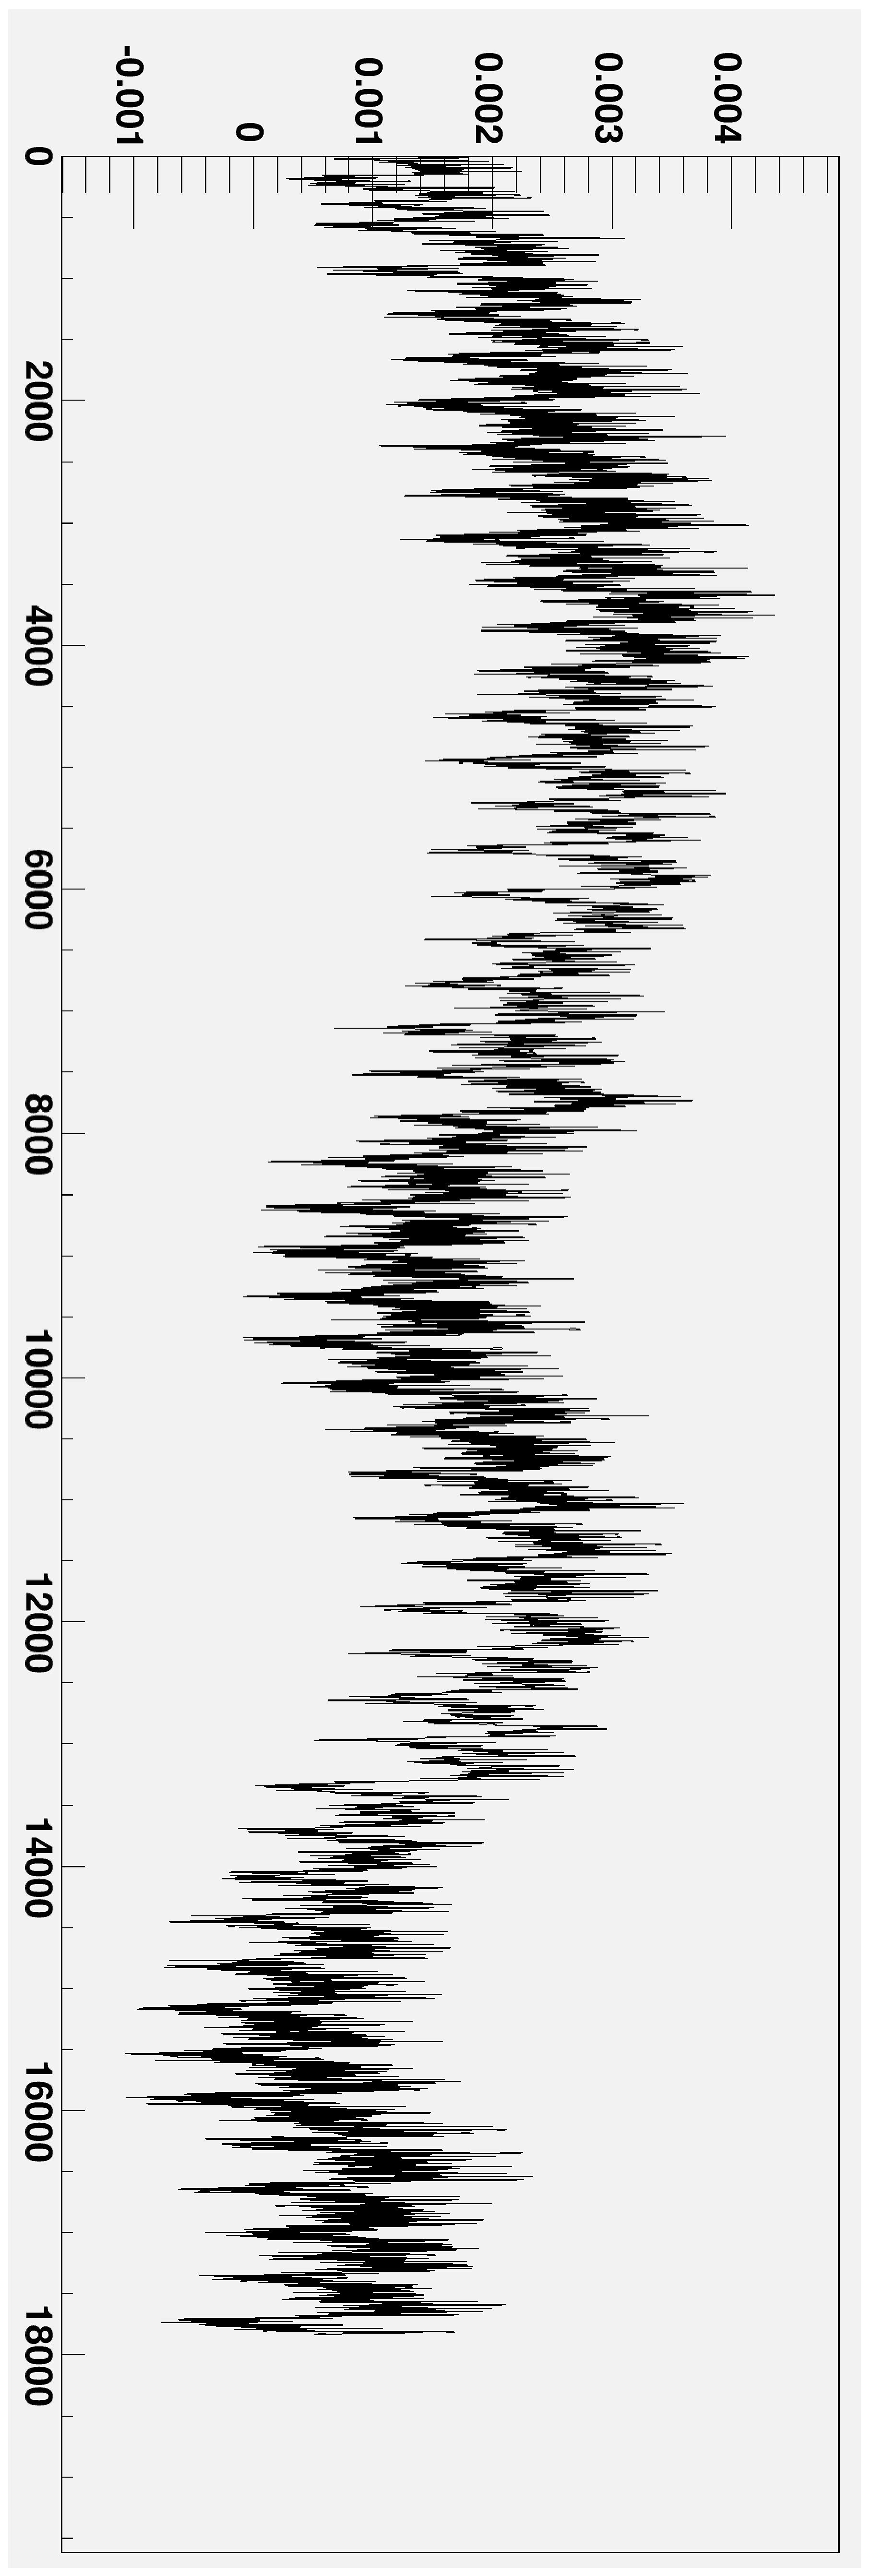
\includegraphics[height=\textheight]{doc/img/lod_g.eps} % width=0.75\textwidth
  \caption{Dane wejściowe, mierzone odstępstwa od długości dnia w sekundach}
  \label{fig:lod_g}
\end{figure}

\begin{figure}[htbp]
  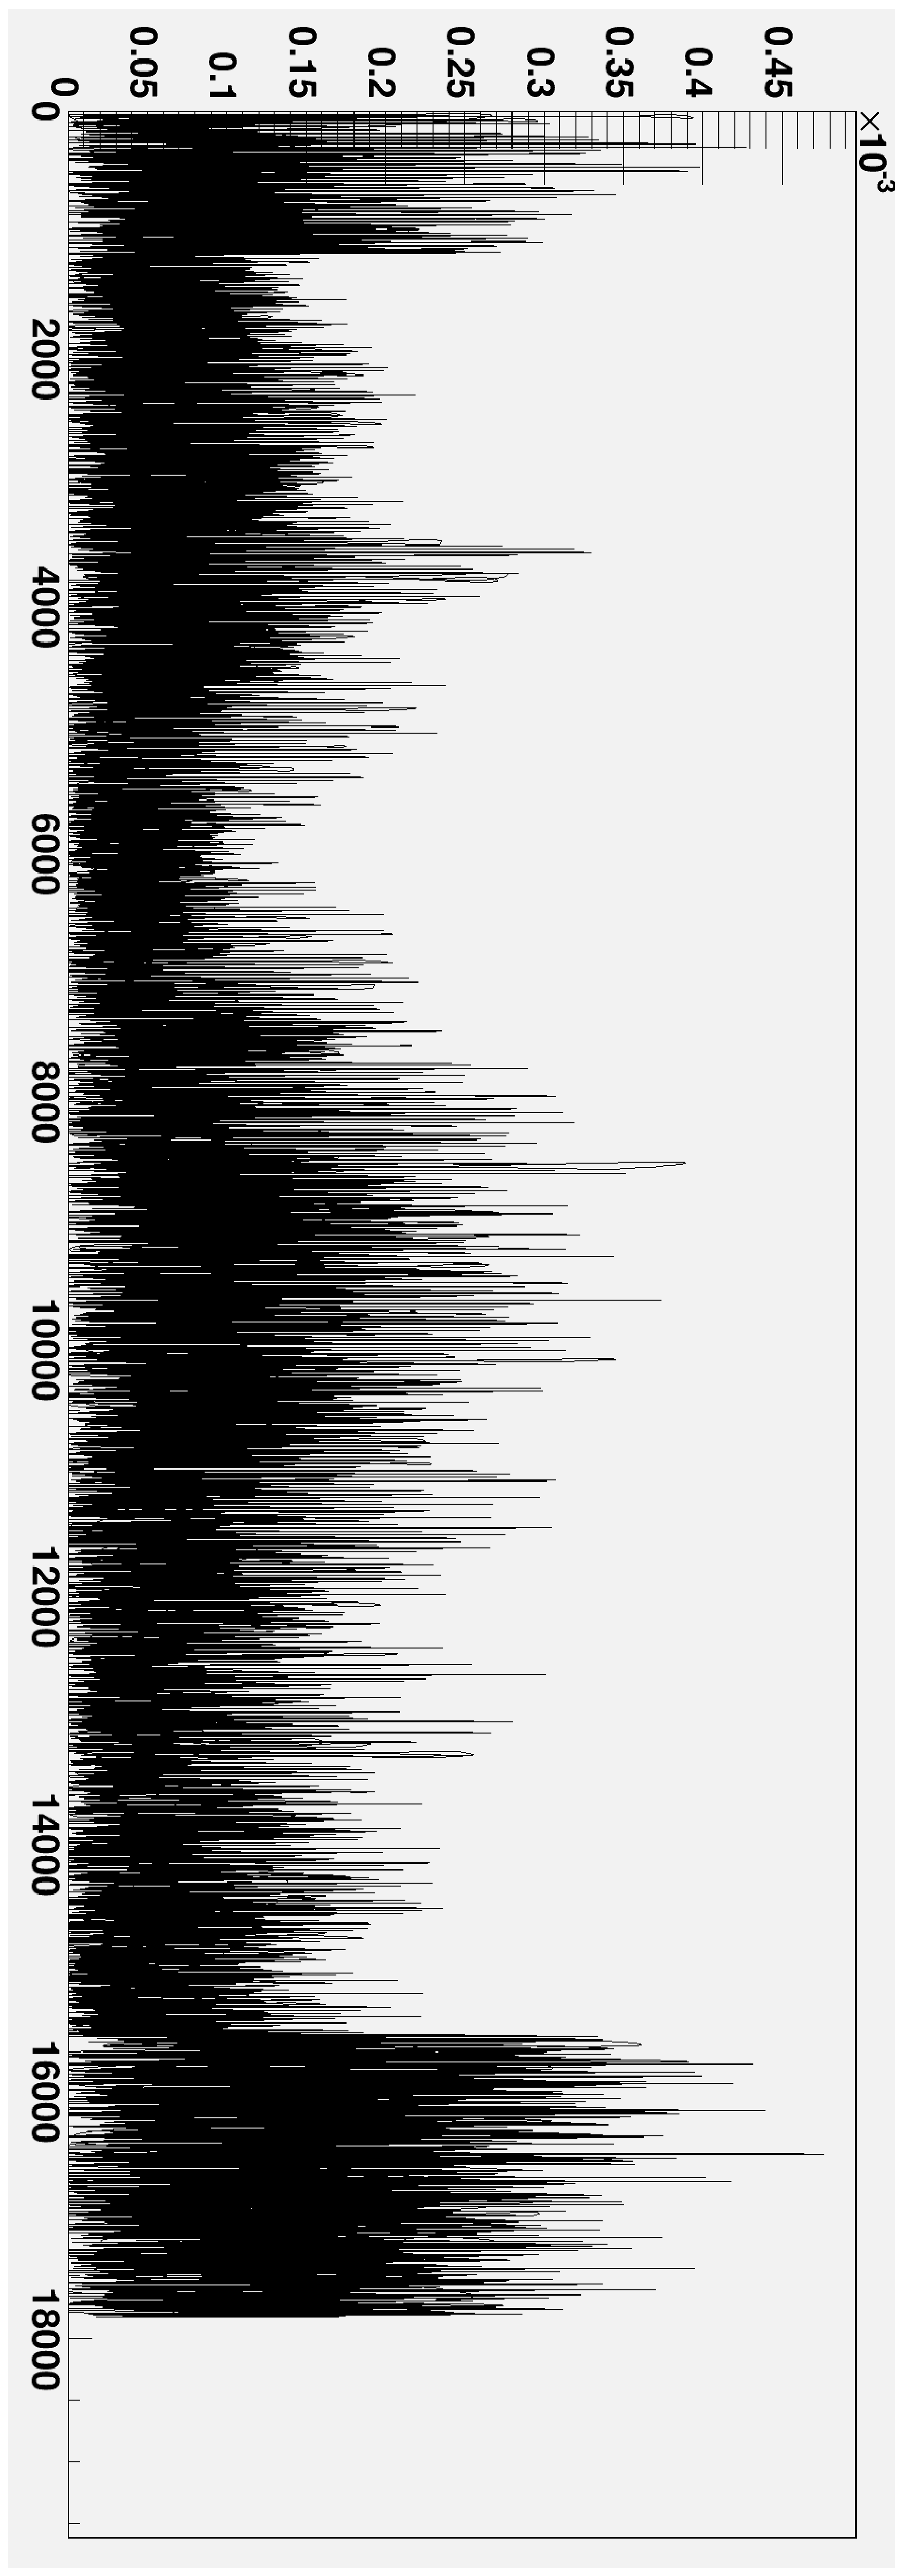
\includegraphics[height=\textheight]{doc/img/err_g.eps}
  \caption{Błąd prognozy odstępstwa od długości dnia w sekundach przy uśrednianiu po różnych topologiach sieci z 15 neuronami}
  \label{fig:err_g}
\end{figure}

\begin{figure}[htbp]
  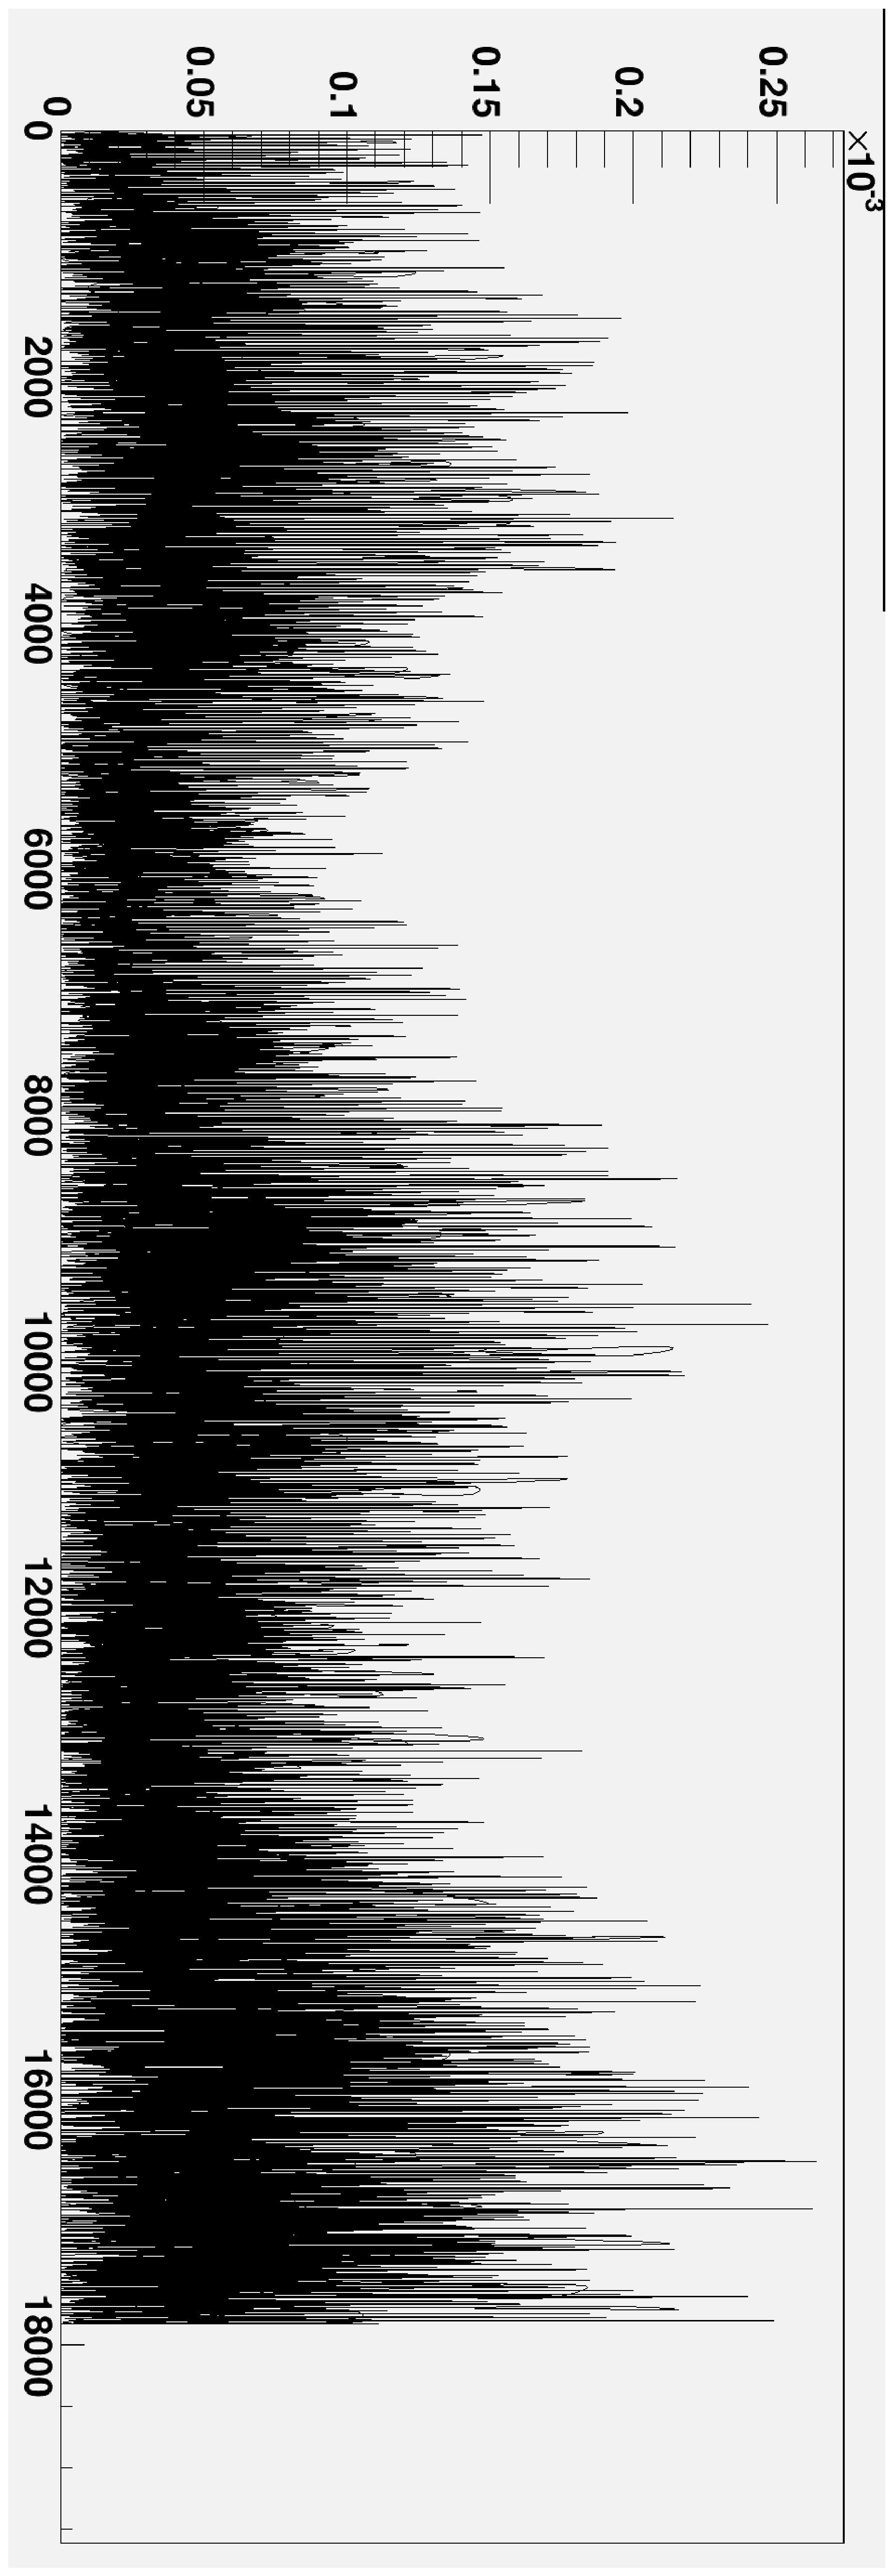
\includegraphics[height=\textheight]{doc/img/err_s.eps}
  \caption{Błąd prognozy odstępstwa od długości dnia w sekundach przy wzięciu najlepszej sieci wybranej z różnych topologii mających 15 neuronów, wybrana siec ma 8 neuronów opóźnienia wejściowego, 3 opóźnienia wyjściowego i 4 w warstwie ukrytej}
  \label{fig:err_s}
\end{figure}


\section{Literatura}
\begin{enumerate}
\item \emph{Sieci neuronowe do przetwarzania informacji}, Stanisław Osowski
\item \emph{Prediction of Earth orientation parameters by artificial neural networks - H. Schuh, M. Ulrich, D. Egger, J. Muller, W. Schwegmann}, Journal of Geodesy (2002) 76: 247-258,\\http://www.springerlink.com/content/vu1fk2krt918u32g/
\item \emph{NN in EOP prediction - M. Kalarus}, http://www.cbk.waw.pl/~kalma/presentations/Application\_of\_NN\_EGU2005.pdf
\end{enumerate}

\end{document}
